\documentclass[../../main.tex]{subfiles}

\begin{document}

\subsection{User interfaces}

  \subsubsection{User interfaces for the customers}

  User interfaces for the customers should be easy to use, thus taking into
  account the needs of people of all ages and possibly with disabilities.

  All the customers need to interact with receipt scanners at the entrance of
  the stores to get access rights. Then, depending on
  the channel that customers want to use to obtain a line-up receipt, they may
  need to interact with additional user interfaces, as described in the
  following paragraphs.

  \paragraph{User interfaces for the customers using IT devices}

  The following mockups can be navigated with elementary interactivity at this \href{https://app.moqups.com/GnQbxBHNrI/view/page/ad64222d5?ui=0}{link}.

  \begin{figure}[H]
    \centering
    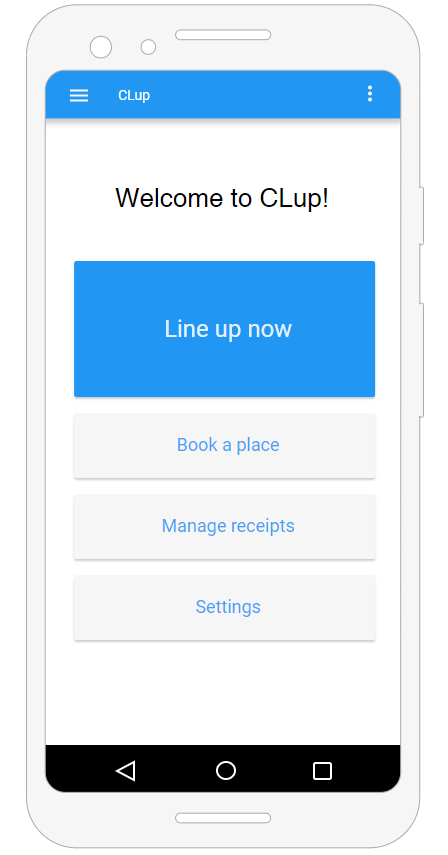
\includegraphics[width=0.5\textwidth]{mockups_01.png}
    \caption{The welcome page.}
  \end{figure}

  \begin{figure}[H]
    \centering
    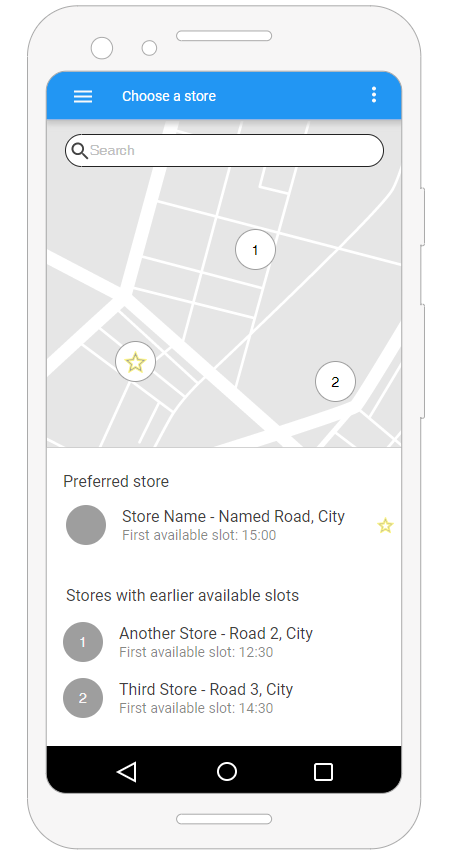
\includegraphics[width=0.5\textwidth]{mockups_02.png}
    \caption{The stores map.}
  \end{figure}

  \begin{figure}[H]
    \centering
    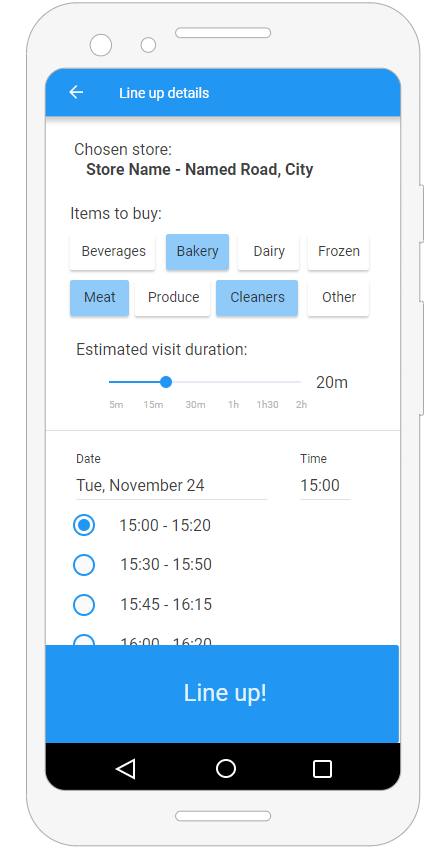
\includegraphics[width=0.5\textwidth]{mockups_03.png}
    \caption{The booking function.}
  \end{figure}

  \begin{figure}[H]
    \centering
    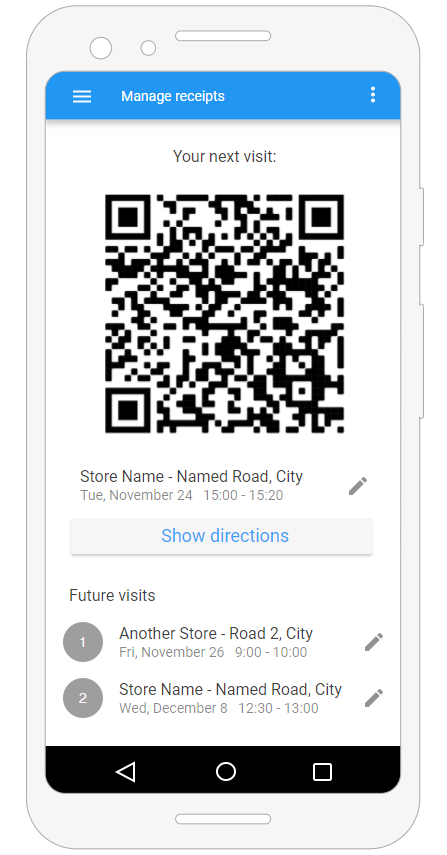
\includegraphics[width=0.5\textwidth]{mockups_04.png}
    \caption{The line up receipt.}
  \end{figure}

  \begin{figure}[H]
    \centering
    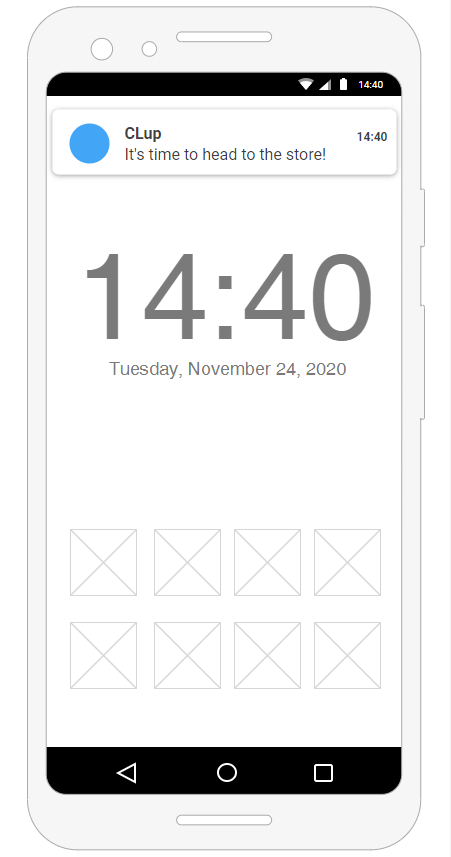
\includegraphics[width=0.5\textwidth]{mockups_05.png}
    \caption{A push notification.}
  \end{figure}

  \pagebreak

  \paragraph{User interfaces for the customers using a standard telephone line}

  Customers using a standard telephone line are allowed to use the system,
  although with limited functionality. Customers can interact with the system by
  calling a dedicated telephone number. An interactive system picks up the call,
  receives input from the customer through speech recognition and DTMF tones
  recognition, and replies to the customer through speech synthetization.

  \paragraph{User interfaces for the customers using the system in presence (fallback method)}

  Customers who cannot use one of the other methods described before can
  interact with the system, with limited functionality, thanks to store
  assistants outside of the stores. The assistants act as a proxy to the system
  for the customers, so no specific user interface is needed for these
  customers.

  \subsubsection{User interfaces for the store assistants}

  Store assistants can interact with the system to generate line up tickets for
  the customers.

  \begin{figure}[H]
    \centering
    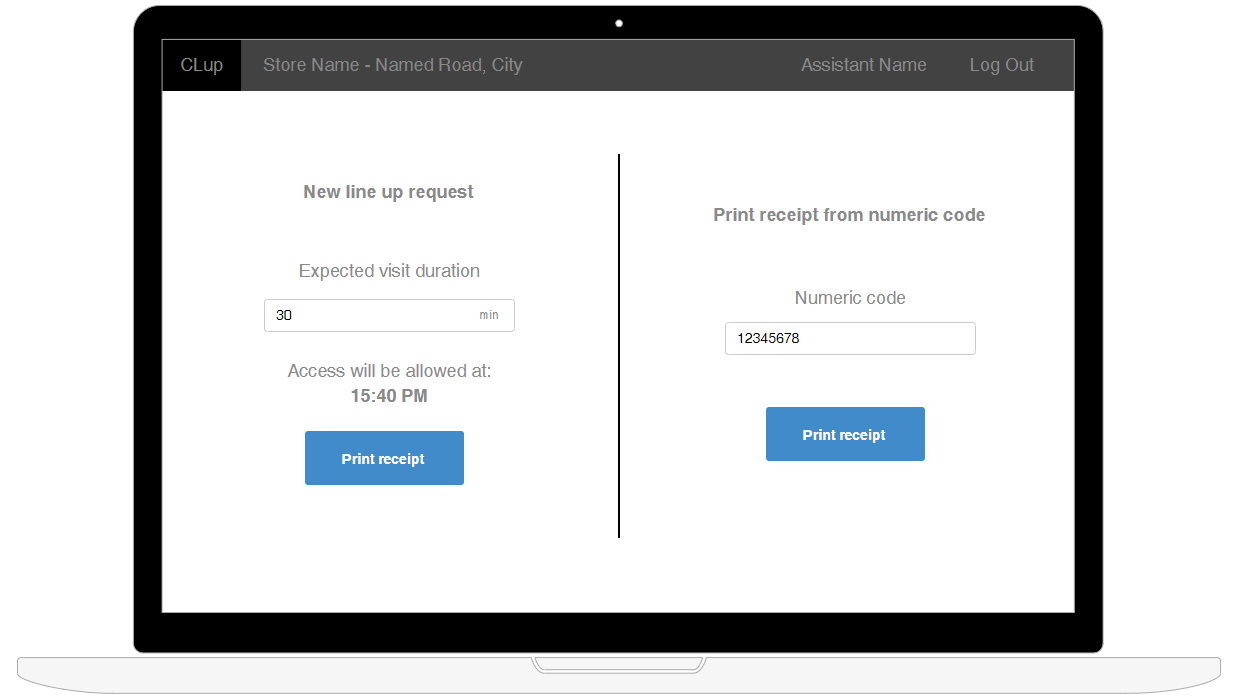
\includegraphics[width=0.75\textwidth]{mockups_06.png}
    \caption{The interface for store assistants.}
  \end{figure}

  \subsubsection{User interfaces for the store managers}

  Store managers can interact with the system to monitor the number of people
  inside the stores and to define limitations on the maximum number of people
  allowed in each department of the store.

  \begin{figure}[H]
    \centering
    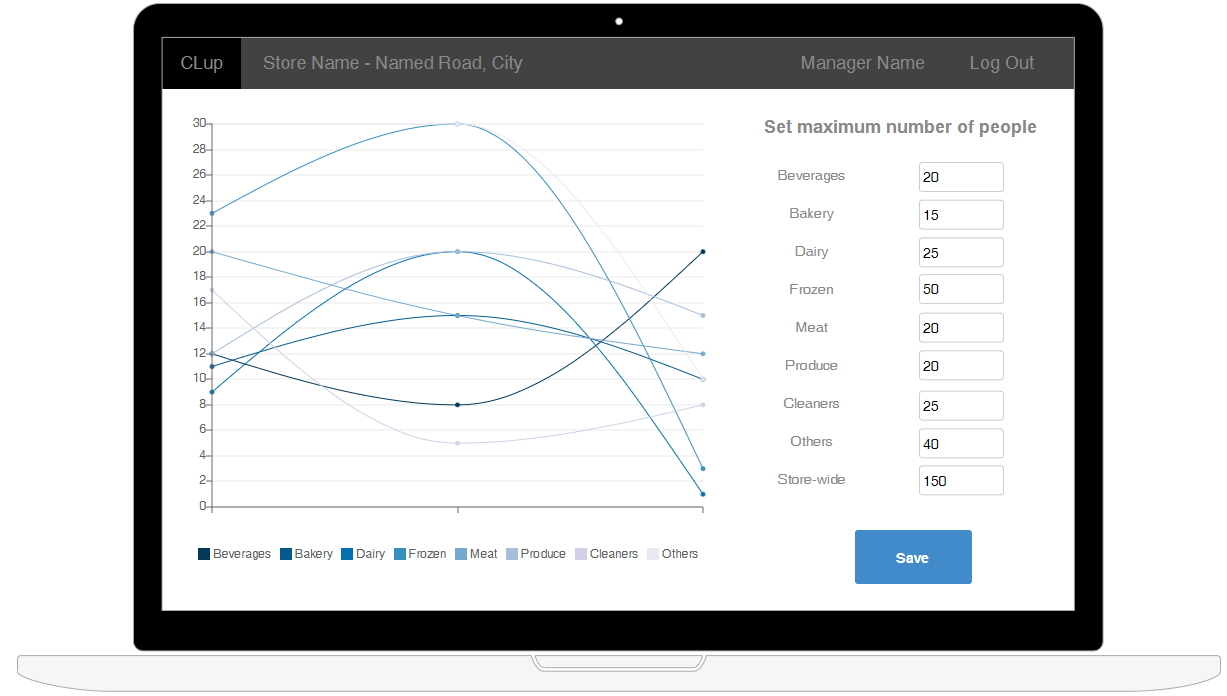
\includegraphics[width=0.75\textwidth]{mockups_07.png}
    \caption{The interface for store managers.}
  \end{figure}

\subsection{Hardware interfaces}

Customers who want to interact with the system with full functionality need to
have an IT device with support for Internet connectivity (mandatory) and able to
provide geolocation information (optional). Customers who do not satisfy this
requirement but still want to interact with the system remotely need to have any
kind of devices that is able to place phone calls to a standard telephone
number.

Store assistants and store managers need to have an IT device with support for
Internet connectivity. Store assistants systems need to interact with printers
placed outside of the stores to print line up receipts for the customers that
initially used a telephone line to interact with the system or for the ones who
chose to use the system in presence, as a fallback.

Moreover, the system interacts with receipt scanners with support for Internet
connectivity. Such devices will be placed at the entrance of the stores and they
will unlock access control devices to let the customers enter. 

Finally, the system interacts with receipt scanners with support for Internet
connectivity placed at the cash counters (both automatic and human-managed) to
register the end of a visit to the store.

\subsection{Software interfaces}

The IT device used by customers who want to interact with the system with full
functionality, by store assistants and by store managers need to either have an
Internet browser with HTML5 capabilities installed, or support the installation
of native apps for the supported platforms (Android, iOS). Depending on the
requirement which is satisfied, the system will use browser APIs or system APIs
to interact with the user upon user request or with push notifications.

The system interacts with the software interfaces of the automatic phone call
provider thanks to which customers can interact via a standard telephone line.

\subsection{Communication interfaces}

Customers who want to interact with the system with full functionality, store
assistants, store managers and the devices that scan the customers' line up
receipt use any kind of Internet connection to communicate with the system.
Devices of customers who want to interact with the system with full
functionality which are able to provide geolocation information use such system
(GPS or equivalent) to retrieve the location. Customers who want to interact
with the system remotely but do not have a suitable IT device use a standard
telephone line to communicate with the system.

The system uses an Internet connection to communicate with the automatic phone
call provider thanks to which customers can interact via a standard telephone
line.

\end{document}
